\documentclass[12pt]{article}

\usepackage{sbc-template}

\usepackage{graphicx,url}

%\usepackage[brazil]{babel}   
\usepackage[utf8]{inputenc}  

     
\sloppy

\title{Classificação de \textit{fake news} utilizando Aprendizado de Máquina}

\author{Murilo Luis C. Neves\inst{1}, Vitor Padovani\inst{1}, Fernando Silva Grande\inst{1}}


\address{Departamento de Informática -- Universidade Estadual de Maringá}

\begin{document} 

\maketitle

\begin{abstract}
  This meta-paper describes the style to be used in articles and short papers
  for SBC conferences. For papers in English, you should add just an abstract
  while for the papers in Portuguese, we also ask for an abstract in
  Portuguese (``resumo''). In both cases, abstracts should not have more than
  10 lines and must be in the first page of the paper.
\end{abstract}
     
\begin{resumo} 
  Este meta-artigo descreve o estilo a ser usado na confecção de artigos e
  resumos de artigos para publicação nos anais das conferências organizadas
  pela SBC. É solicitada a escrita de resumo e abstract apenas para os artigos
  escritos em português. Artigos em inglês deverão apresentar apenas abstract.
  Nos dois casos, o autor deve tomar cuidado para que o resumo (e o abstract)
  não ultrapassem 10 linhas cada, sendo que ambos devem estar na primeira
  página do artigo.
\end{resumo}

\section{Introdução}

Falar um pouco sobre fake news e aprendizado de máquina...

\section{Fundamentação Teórica}

\subsubsection{Random Forest}

\subsubsection{Logistic Regression}

\subsubsection{Gradient Boosting}

\subsubsection{Redes Neurais}

\section{Materiais e métodos}

	Nesta seção, são descritos os materiais utilizados para o trabalho (seção \ref{sec:materiais}) e os métodos como foram trabalhados (seção \ref{sec:metodos}).
	
\subsection{Materiais} \label{sec:materiais}

Os materiais utilizados para esse trabalho incluem o \textit{dataset} WELFake, e, como ferramentas de codificação principais, as bibliotecas \textit{Scikit-Learn} e \textit{Torch}.

\subsubsection{Base de dados}

O \textit{dataset} utilizado é o WELFake, devido ao grande volume de dados presentes no mesmo e um relativo balanceamento entre as classes real e falso. Ele possui 72134 entradas, onde 35028 são reais e 37106 são falsas. No entanto, como é mostrado na seção \ref{sec:preproc}, há duplicatas, o que torna o número de entradas válidas no \textit{dataset} menor.

O \textit{dataset} possui como colunas o identificador de cada texto, título, texto e \textit{label}, onde a \textit{label} 0 indica notícia falsa e 1 indica notícia real. Um ponto importante de ser notado é que, como o \textit{dataset} não possui \textit{features} pré-extraídas (apenas possui o texto em si), elas foram posteriormente extraídas pelos discentes (seção \ref{sec:preproc}).

Uma análise inicial indica a seguinte proporção de duplicatas:

\begin{table}[h]
	\centering
	\begin{tabular}{|l|c|}
		\hline
		Duplicatas em títulos & 9786 \\
		Duplicatas em textos & 9415 \\
		Duplicatas em linhas inteiras & 8456 \\
		\hline
	\end{tabular}
	\label{tab:duplicatas}
	\caption{Quantidade de duplicatas encontradas na base de dados}
\end{table}

Para este trabalho, considerou-se que apenas duplicatas tanto em título quanto em textos deveriam ser removidas. Alguns gráficos que mostram a distribuição dos tamanhos dos textos e títulos seguem.

\begin{figure}[h]
	\centering
	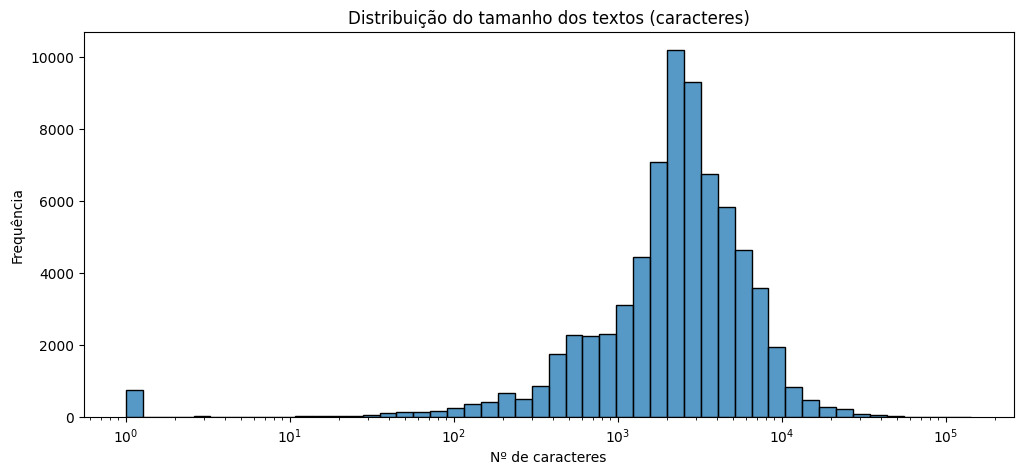
\includegraphics[width=0.6\linewidth]{imagens/preproc/tamanho_textos_char.png}
	\caption{Distribuição dos tamanhos dos textos (em caracteres)}
	\label{fig:preproc_tam_txt_char}
\end{figure}


\begin{figure}[h]
	\centering
	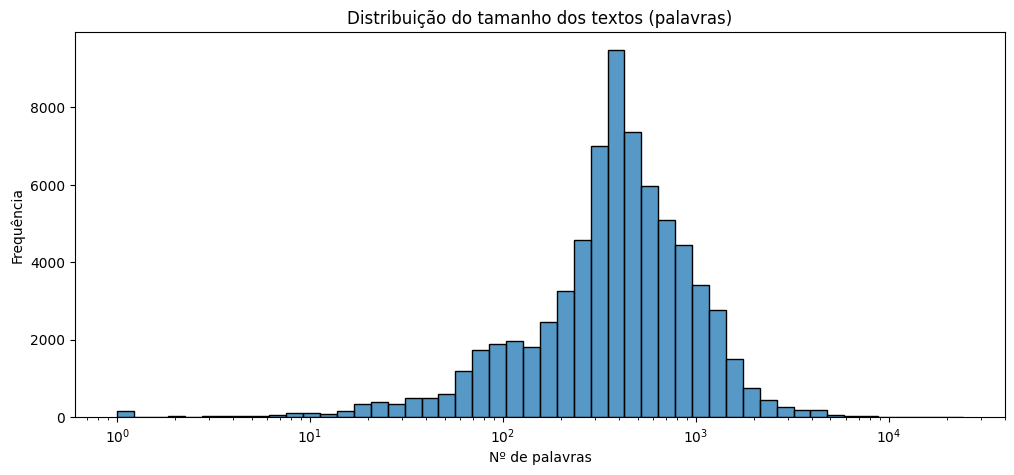
\includegraphics[width=0.6\linewidth]{imagens/preproc/tamanho_textos_palavras.png}
	\caption{Distribuição dos tamanhos dos textos (em palavras)}
	\label{fig:preproc_tam_txt_pal}
\end{figure}


\begin{figure}[h]
	\centering
	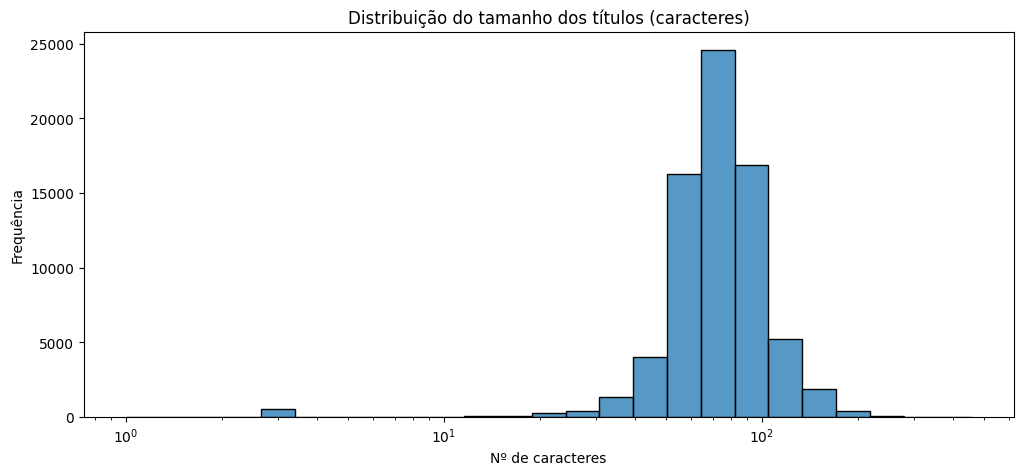
\includegraphics[width=0.6\linewidth]{imagens/preproc/tamanho_titulos_chars.png}
	\caption{Distribuição dos tamanhos dos títulos (em caracteres)}
	\label{fig:preproc_tam_tit_char}
\end{figure}

\subsubsection{Scikit-Learn}

\subsubsection{Torch}

\subsection{Métodos} \label{sec:metodos}

\subsubsection{Pré-processamento} \label{sec:preproc}

\subsubsection{Método 1: Técnicas clássicas}

\subsubsection{Método 2: Redes neurais}

c. Metodologia contendo uma descrição das características da base de dados selecionada,
os métodos aplicados, bem como da métrica de avaliação utilizada para verificar a
qualidade dos métodos aplicados;

\section{Resultados}

\section{Conclusões}

\bibliographystyle{sbc}
\bibliography{sbc-template}

\end{document}
